%Introduction

\section{Abstractions}

The architecture of the \textsc{Test Stand} consists in at leas three stand alone modules, that establish a mono-directional communication flow. But what exactly is a module? Chapter \ref{chap:heaven} reports some requirements which directly affect the implementation experience of \namens : [R.10] i.e. the need of an \textit{Extendible Design} and [R.11], which states the necessity of an \textit{Event-base architecture} to properly face RSPEngines,  which usually exploit this communication pattern.

Developing an \textit{Extendible} \textsc{Test Stand} to handle any RSP Engine requires two abstractions:
\begin{itemize}
\item \textit{Event}
\item \textit{Event Processor}
\end{itemize} 

The \textit{Event} is required to build a hierarchical communication. \textsc{Test Stand} handle many events flows, a lest three: one for the RSP Engine module, one for the communication between modules and one to communicate with the user. Next section about data clarify how the communication is structured and we detail consequently how the components communicates. The \textit{Event Processor} guarantees the system to be modular, it simplifies the behaviour of each component of the \textsc{Test Stand} structure, stereotyping the way of interaction. 

Thus, to answer the question above, a module is an \textit{Event Processor} which can be positioned everywhere in the pipeline which represent the \textsc{Test Stand} architecture. 
As a matter of facts, specific implementations of modules reduce the generality of this definition and also the flexibility of the modules themselves.	

Last but not least the the requirement [R.4] states the \textsc{Test Stand}\textit{ must not be running when the RSP Engine is under execution} (see Section \ref{sec:requirements}. We think the system as a Finite State Machine (FSM) and its modules are FSM too.

Each module can work only if its current state allow processing. An Error State prevents the propagation on errors in the data. The following schema represent the FSM for all the modules of \name, even the Baselines, and solo for its external structure, which exploit this behaviour to control execution an stop its process while the RSPEngine is running.

\begin{figure}[tbh]
  \centering
	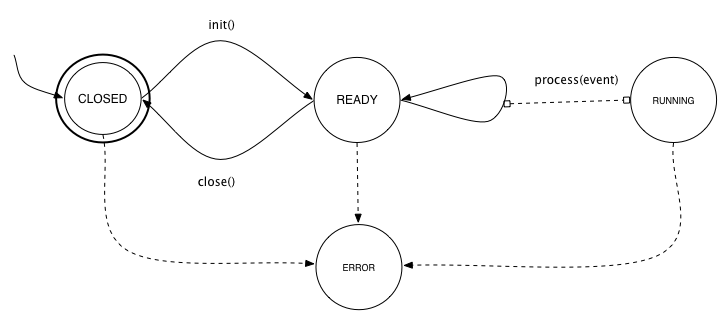
\includegraphics[width=\linewidth]{images/fsm-schema}
	\caption{Module Finite State Machine Automata} 
  	\label{fig:module-fsm}
\end{figure}


\section{Events and Data}\label{sec:data-impl}

\begin{figure}[tbh]
  \centering
	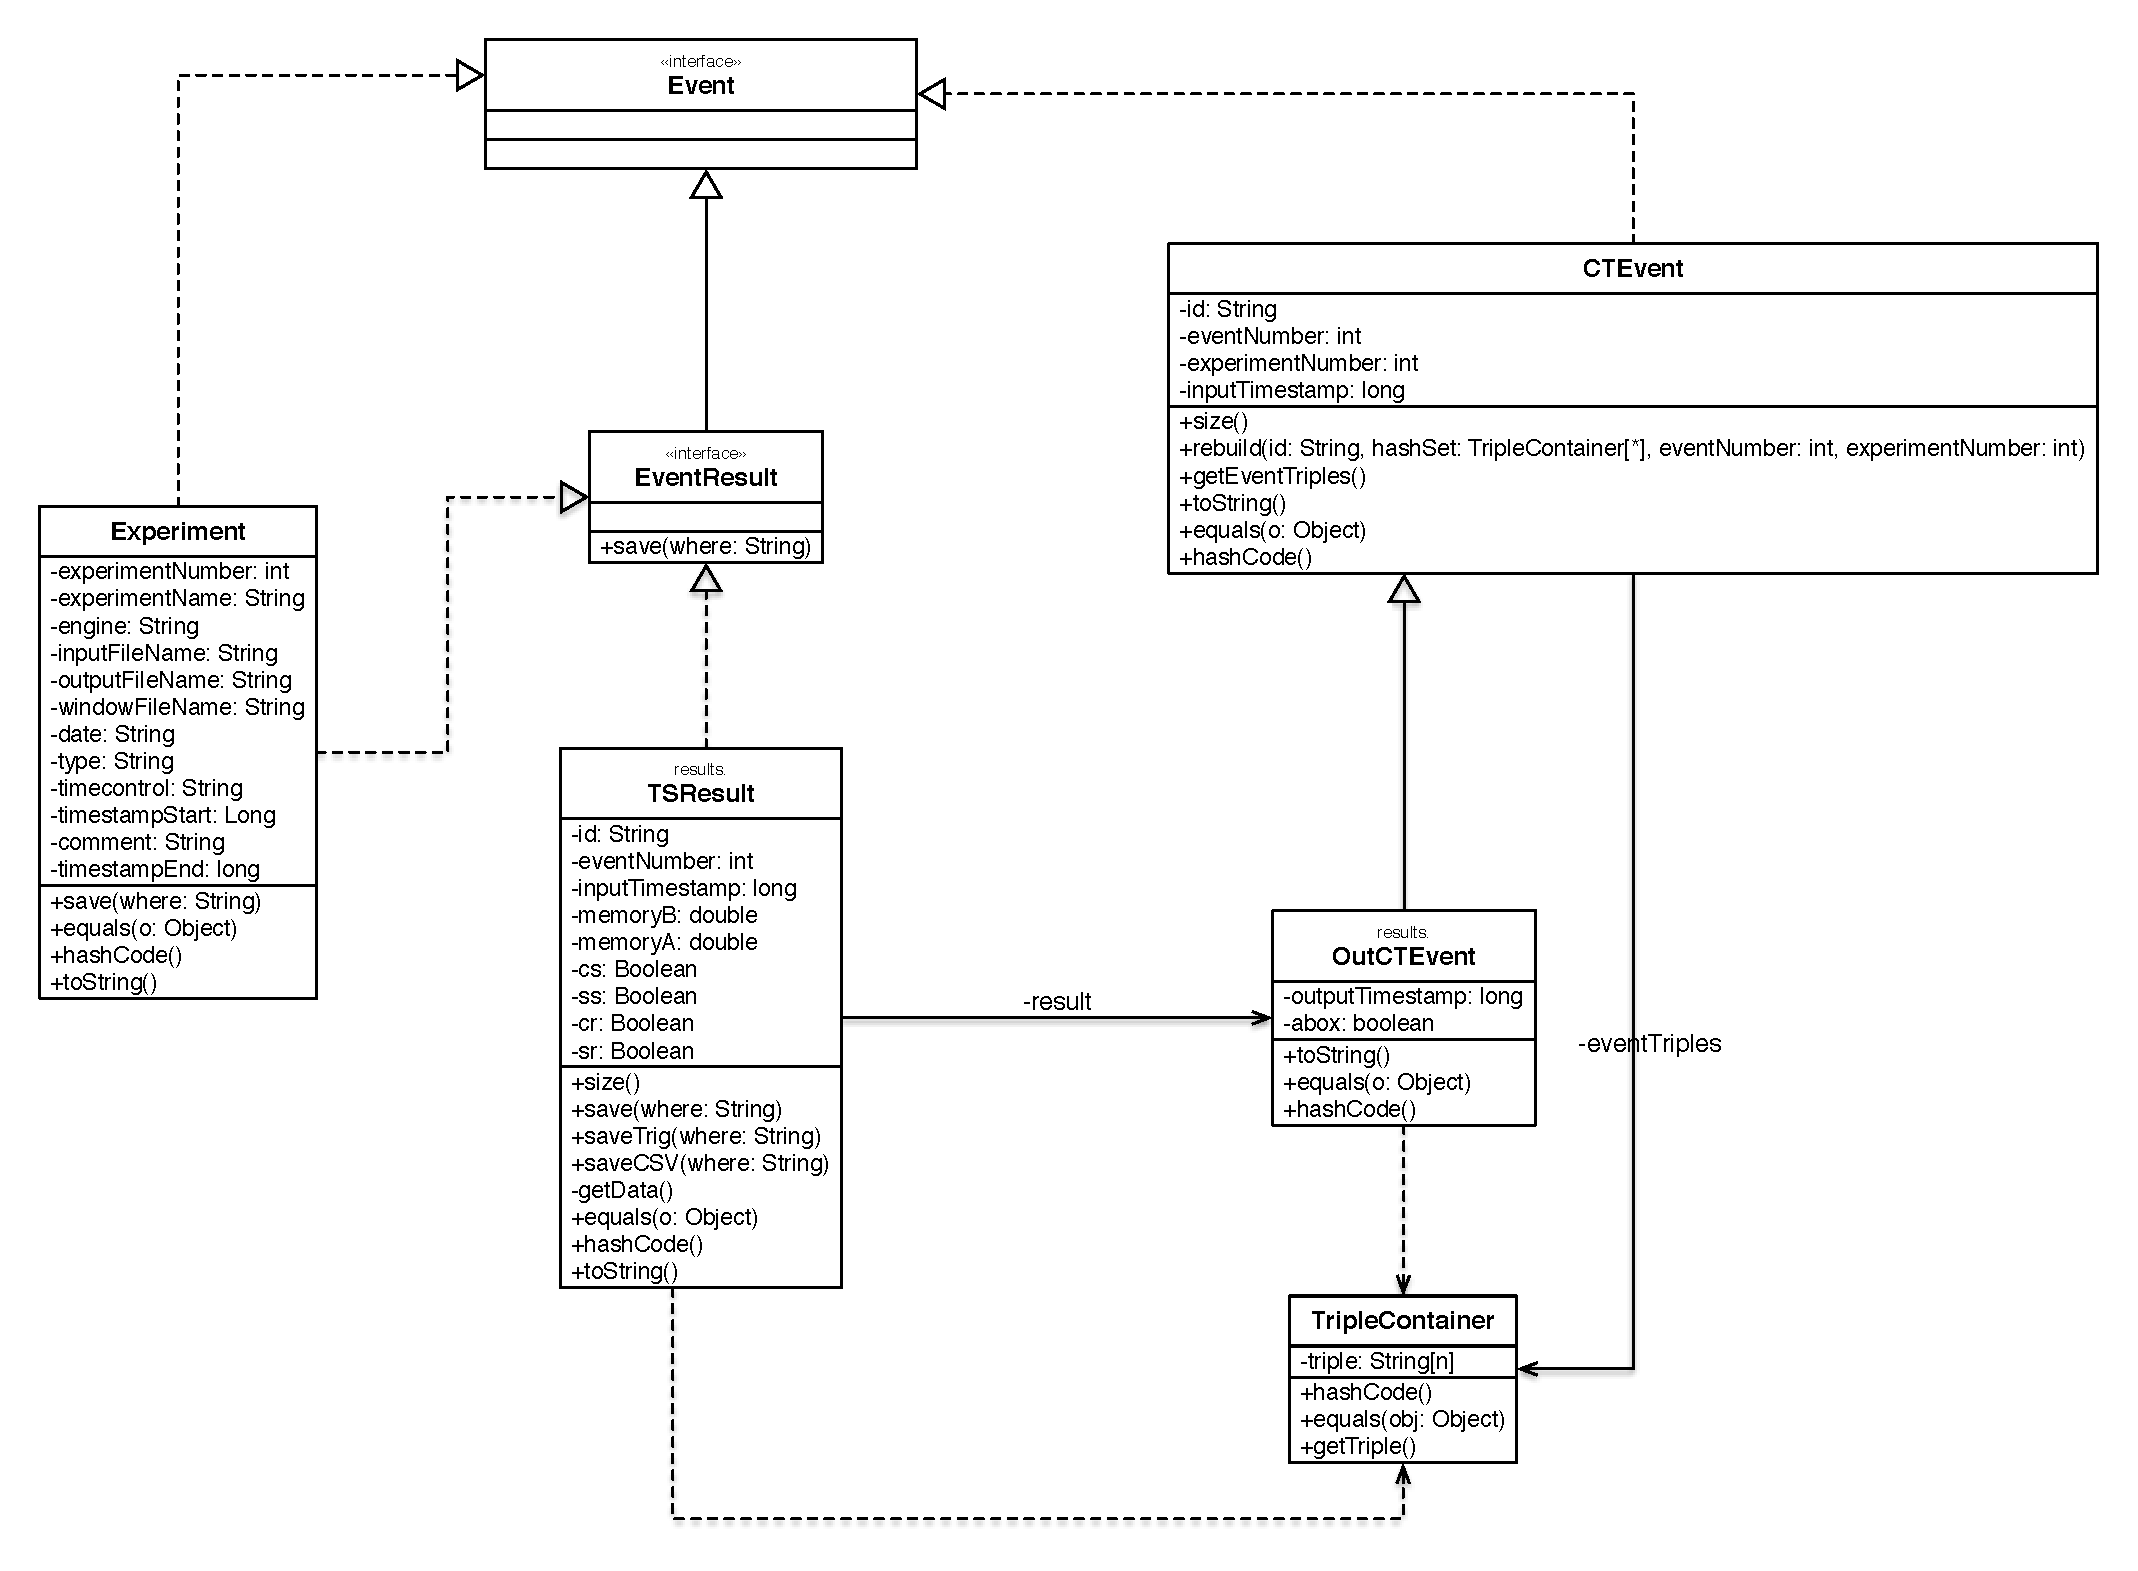
\includegraphics[width=\linewidth]{images/uml_events}
	\caption{UML Schema for all the events involved in the system} 
  	\label{fig:module-fsm}
\end{figure}

Chapter \ref{chap:problem-setting} poses the requirements of an Event-based architecture [R.11] for the \textsc{Test Stand} to properly handle the interaction with an event-based system like RSP Engines. Moreover, Chapter \ref{chap:heaven} describes \name workflow and how it exchange events during the execution. The \textsc{Test Stand} establishes a mono-directional communication flow between its components. The modules exchanges events which are actually data at different points of the process.
The \name handle in general three kind of events:
\begin{enumerate}
\item \textbf{Experiment} - represents the tuple $<\mathcal{E}, \mathcal{D},\mathcal{T},\mathcal{Q}>$ and all the experiment metadata.
\item \textbf{CTEvent and OutCTEvent} - contains a set of triple which has the same timestamp, the OutCTEvent rapresent the event produced by the RSPEngine after processing the active window
\item \textbf{TSResult} - wraps the OUTCTEvent adding the information about the minimal sensor data: memory and latency and complete and soundness if it evaluated at runtime (see Section \ref{sec:requirements})
\end{enumerate}

The Experiment must be created and passed to the Test Stand. \name requires a setup phase to prepare experiments. At this moment we exploits a property file which contains all the information we build the Experiment from. 

The requirement [R.12] demands an \textit{Easy-to-Parse RDF Serialisation for the events presented to the RSP Engine in exam}, The CTEvent and the OutCTEvent carry RDF triples in NT-Triple\footnote{http://www.w3.org/2001/sw/RDFCore/ntriples/}, which is the easiest RDF serialisation to parse. RDF Triples are stored in the events into the TripleContainer class, we develop exploit this wrapper in order to redefine the triple hashcode and equals method guaranteeing their uniqueness inside an event.

\section{Modules}

\subsection{Streamer}	\label{sec:streamer-impl}
\begin{figure}[tbh]
  \centering
	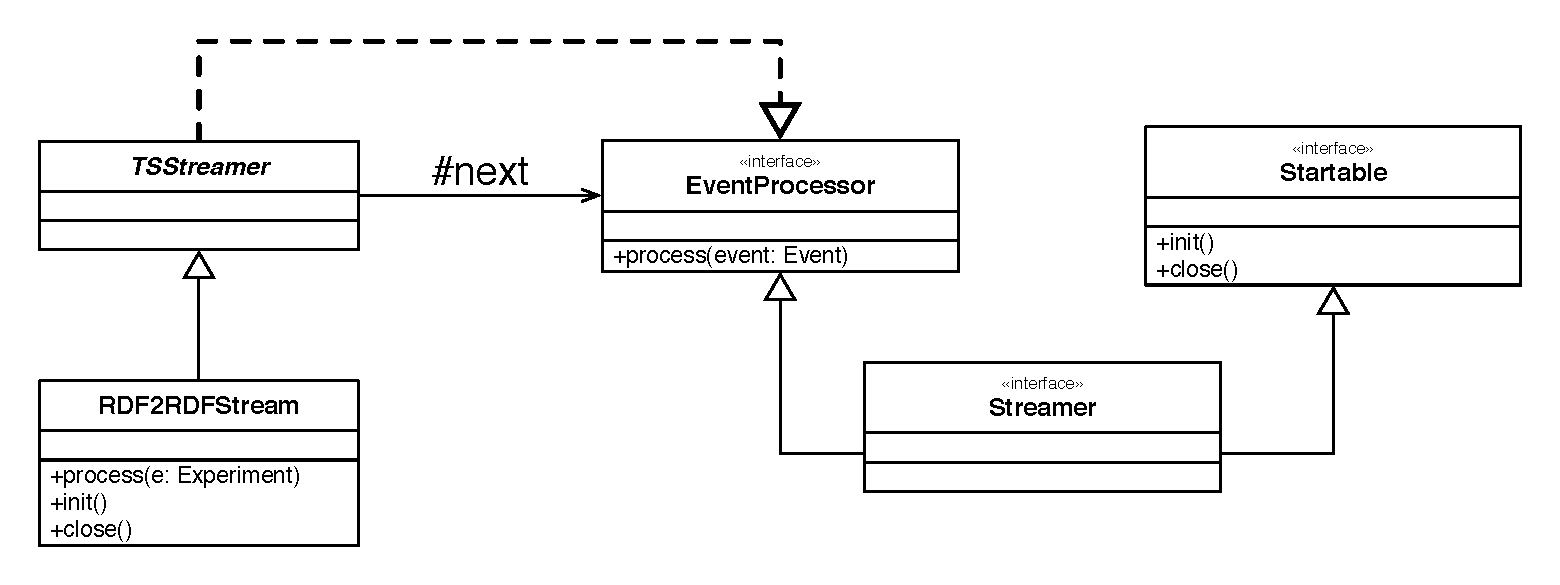
\includegraphics[width=\linewidth]{images/uml_tstreamer}
	\caption{Streamer UML Schema with TSStreamer and Implementation example} 
  	\label{fig:tsstreamer}
\end{figure}

The most general implementation of the \textsc{Streamer} is the on TSStreamer, which is the head-module in the \textsc{Test Stand} pipeline. It processes an Experiment and communicates in general with one Event Processor, which instead process CTEvent. The way  how the TSStreamer implementation communicates with the following EventProcessor may changes to follow the user needs. 
Chapter \ref{chap:evaluation} contains the experimental setting we follow to execute our experiment. It is worth to note that we use LUBM Benchmarks to generate the data for the experiments. For this reason, in order to build an RDFStream starting from the static data produced by LUBM we developed the RDF2RDFStream module.

\begin{figure}[tbh]
  \centering
	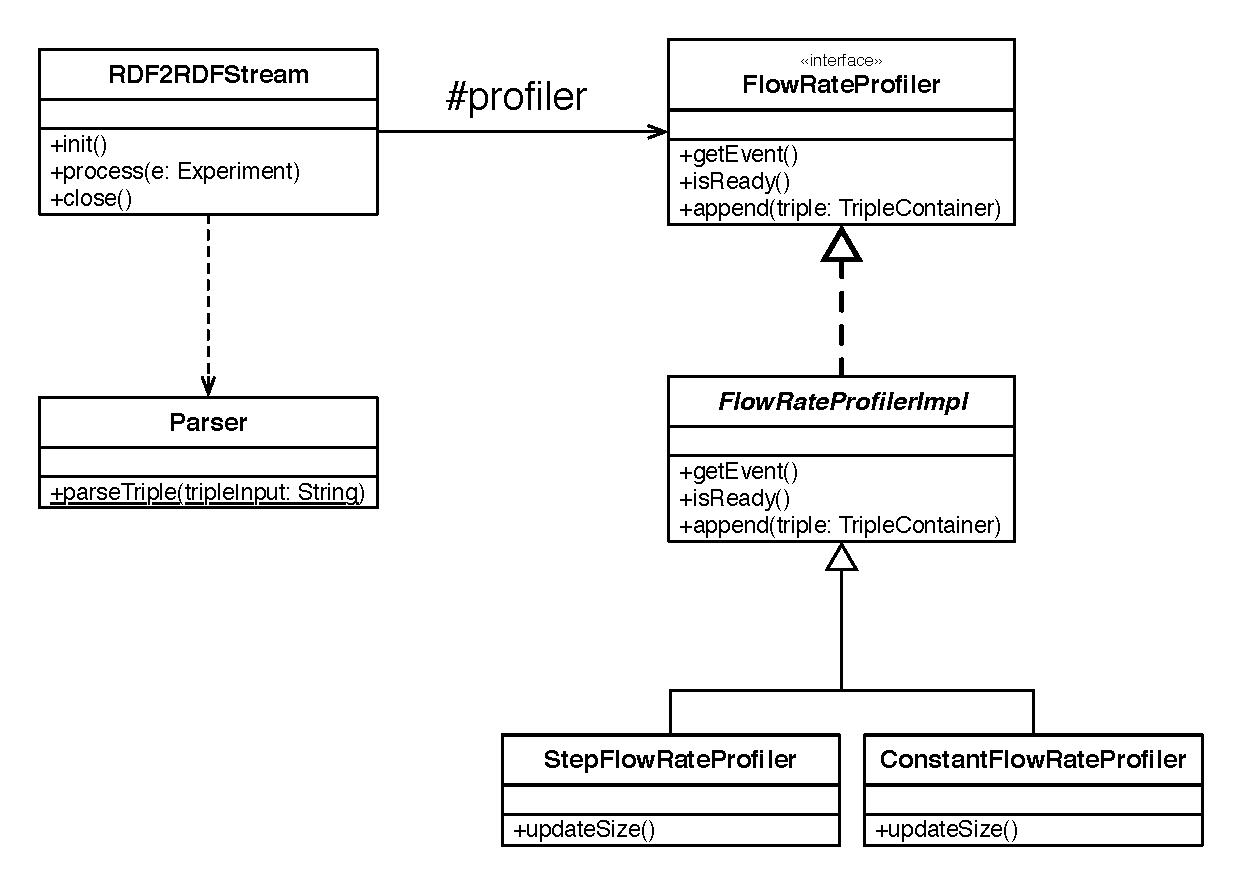
\includegraphics[width=\linewidth]{images/uml_flowrateprofiler}
	\caption{RDF2RDFStream and Flow Rate Profiler UML Schema} 
  	\label{fig:flowrateprofiler}
\end{figure}


The RDF2RDFStream exploits two components a Parser and the FlowRateProfiler. The Parser reads in memory one by one the triples in the file, guaranteeing data independence [R.1]. The file is generated by LUBM(1000,0), which means 1000 different universities with random generation seed 0. In this way, also RDF2RDFStream satisfies requirement [R.5] by allocating only the memory necessary to parse a triple. The Flow Rate Profiler determines the number of triples to add to a CTEvent and builds such an event. In this way, RDF2RDFStream can generate different RDF streams $\mathcal{D}$, which differentiate on the number of contemporary triples in the stream. FlowRateProfiler builds the triple according with a function $y=f(x)$ where $x$ is the number of the CTEvent and the $y$ is the number of this CTEvent will contain. Practically $f$ can be any function from N to N. We develop two FlowRateProfiler for our experiment: 
\begin{itemize}
\item ConstantFlowRateProfiler, which maintains the same number of triples for each events over all the experiment  
\item StepFlowRateProfile, which has a constant number of triple for max $x$ CTEvents, then suddenly changes the number of triple $y$.
\end{itemize}
Other implementations are available in \name right now, but are not used in the experiments:
\begin{itemize}
\item LinearStepFlowRateProfile, which stream $x$ CTEvents of dimension $y$, in terms of triples, then linearly increase the number of a quantity $n$.
\item ConstantRandomFlowRateProfiler, which changes $y$ and $x$ according with two random generators directed by two seeds.
\end{itemize}

\subsection{Result Collector} 

\begin{figure}[tbh]
  \centering
	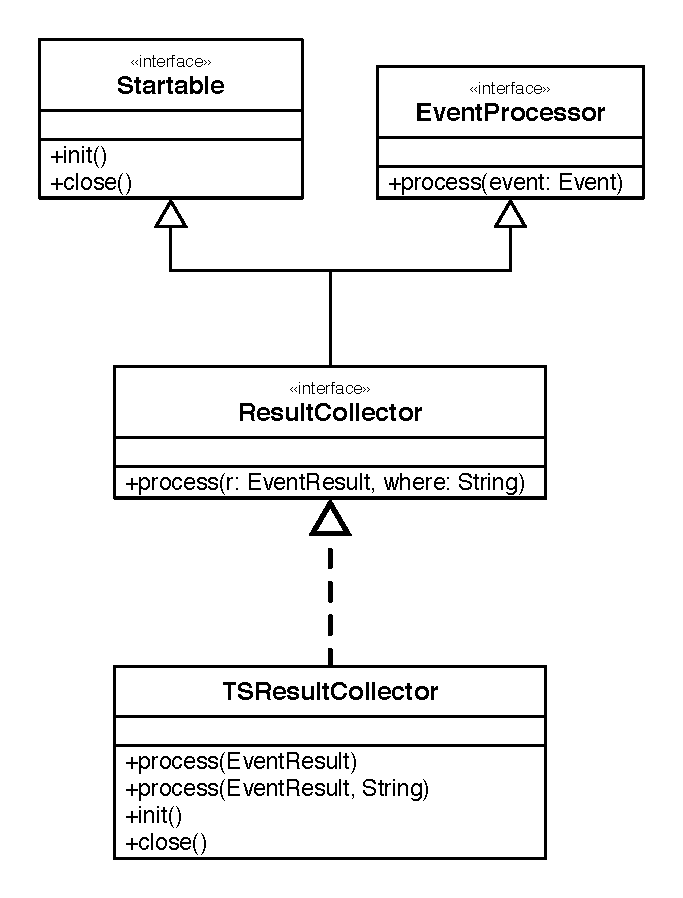
\includegraphics[width=\linewidth]{images/uml_resultcollector}
	\caption{ResultCollector UML Schema with events Experiment, TSResult and OutCTEvent} 
  	\label{fig:resultcollector}
\end{figure}

The ResultCollector realises the acquisition system we need to collect query results data and the one gathered by the \textsc{Test Stand} during the execution. The TSResultCollector implements the ResultCollector  and it is positioned at the end of the pipeline which compose the \textsc{Test Stand}. It is responsible of the saving procedure described above, the requirement [R.7] demands to \textit{enable users extensions with new software sensors and specific measurements collection}, for these reason we need a general saving procedure which does not care about the format of the data. We exploit the \textbf{Active Event Pattern}: each event shares the ssame interface which  expose a method that hides the procedure, leaving to the provider of the event the responsibility to implement the saving procedure according which his needs. The TSResultCollector calls this method over all the events passed to it during the execution. The current implementation the TSResultCollector handles two kind of events, which saving procedures are:
\begin{itemize}
\item TSResult - it saves the data of the query results into a TriG\footnote{http://www.w3.org/TR/trig/} file where the graph key is the event id inside the experiment, while it save the sensor data into a CSV\footnote{$http://en.wikipedia.org/wiki/Comma-separated_values$} file. 
\item Experiment. It saves the experiment metadata and the tuple $<\mathcal{E},\mathcal{D},\mathcal{T},\mathcal{Q}>$ as description field into SQLite\footnote{https://sqlite.org/} database.
\end{itemize} 

\subsection{Test Stand Supporting Structure}\label{sec:teststand}


\begin{figure}[tbh]
  \centering
	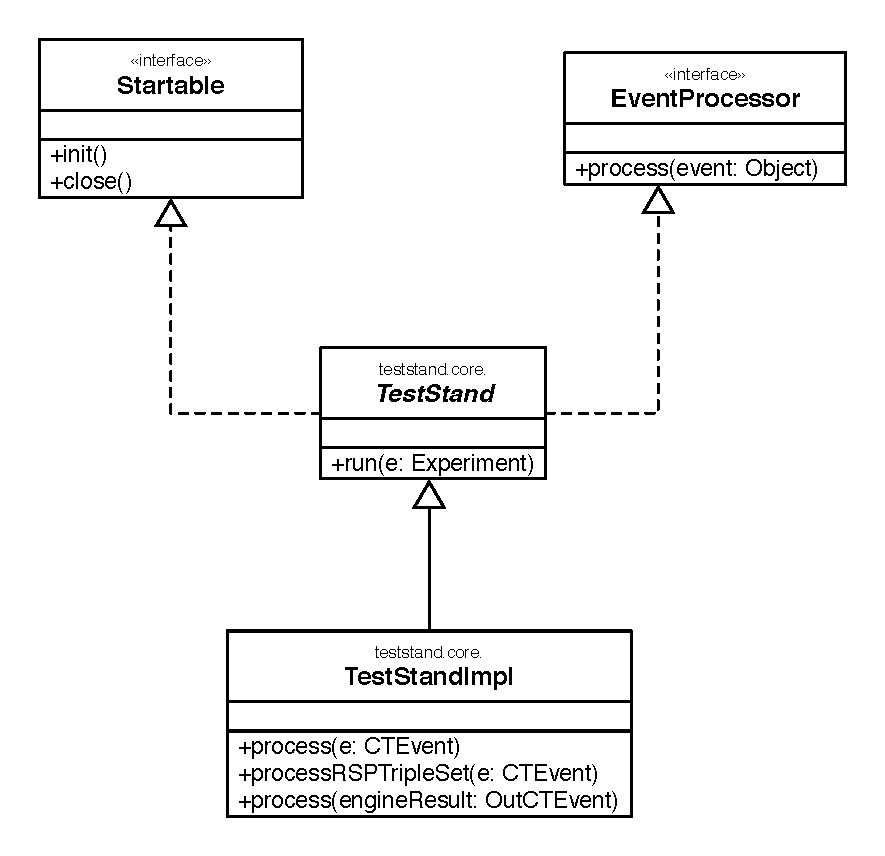
\includegraphics[width=0.5\linewidth]{images/uml_teststand}
	\caption{UML Schema the TestStand} 
  	\label{fig:module-fsm}
\end{figure}


We have described \name \textsc{Test Stand} as set of modules which interact exchanging events during the execution. However, Chapter \ref{chap:havean} describes at the design level the presence of an external structure which orchestrates the communication between the \textsc{Streamer} the \textsc{RSP Engine} and the \textsc{ResultCollector}. The class which allow the modules to communicate and exposes the APIs for users interaction is call TestStand and its current implementation is the TestStandImpl.
Trough an initialisation class which receives the configuration file, the TSStreamer [R.1] the \textsc{RSP Engine} [ R.2 and R.3] and the TSResultCollector are referenced to the TestStandImpl. Once the set-up phase is complete the TestStandImpl is initialized, and it consequently initialises all the upstanding modules, then it receives the Experiment and starts the execution. The TestStand structure is and EventProcessor as the modules mounted on it, and can handle the same events of the TSStreamer and the TSResulCollector.

\begin{figure}[tbh]
  \centering
	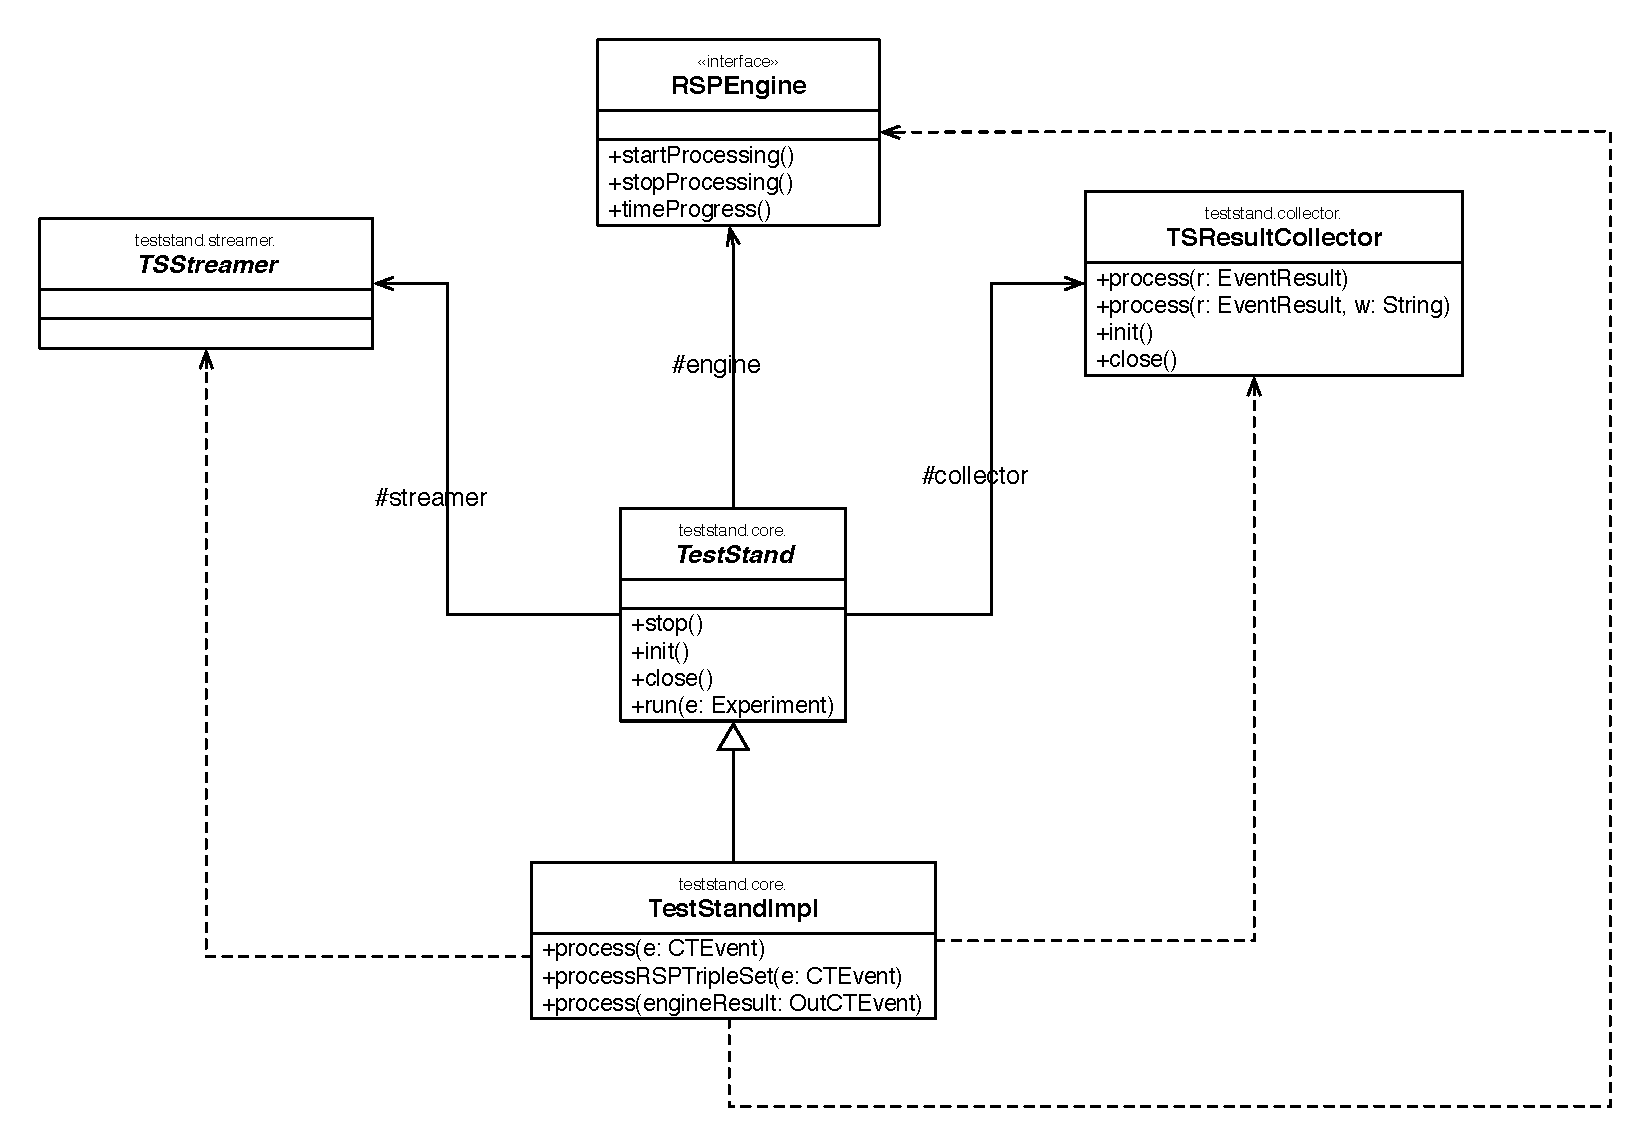
\includegraphics[width=0.90\linewidth]{images/uml_teststand_modules}
	\caption{UML Schema the TestStand with the upstanding modules: TSStreamer, RSPEngine, TSResultCollector} 
  	\label{fig:module-fsm}
\end{figure}

During the execution TestStandImpl intercepts the CTEvents form the Streamer to the RSP Engine as described in Section \ref{sec:arch-workflow}. According with the Experiment specification the TestStandImpl turn off its sensors,. It calculates latency starting a timer when the CTEvent arrives and stopping the timer when it RSP Engine outputs the results. It calculates memory in asking to the JVM in both the point above [R.6]. To fulfil requirements [R.7] any new measurement can be positioned between this two phases of interaction, when the RSP Engine is not running yet or when it has finished the computation. Once the OutCTEvents comes form the RSP Engine, the TestStandImpl wraps it with a TSResult and set the query results data together with the measures to the ResultCollector fulfilling [R.8] and supporting [R.9] for further analysis with the Analyser.
%
%R.6 include basic set of performance measurements [?].
%R.7 enable users extensions with new software sensors and specific measure-
%ments collection.
%R.8 support performance measurements collection for further analysis.

\section{Baselines}\label{sec:baselines-impl}

\name Baselines are four elementary implementation of an RSP Engine which follow the design proposal presented in Section \ref{sec:baselines}, covering [R.13]. They pipeline Esper\footnote{$http://www.espertech.com/esper/$}, a mature commercial DSMS, with the Jena general purpose rule engine\footnote{http://jena.apache.org/documentation/inference/\#rules
}, a flexible reasoning engine. The motivations behind the choice of Esper and Jena regards the intention to fulfil requirement [R.14], baselines Eligibility, coupling this two good solution for reasoning and CEP, to obtain a fair solution the SR context. 

\begin{figure}[tbh]
  \centering
	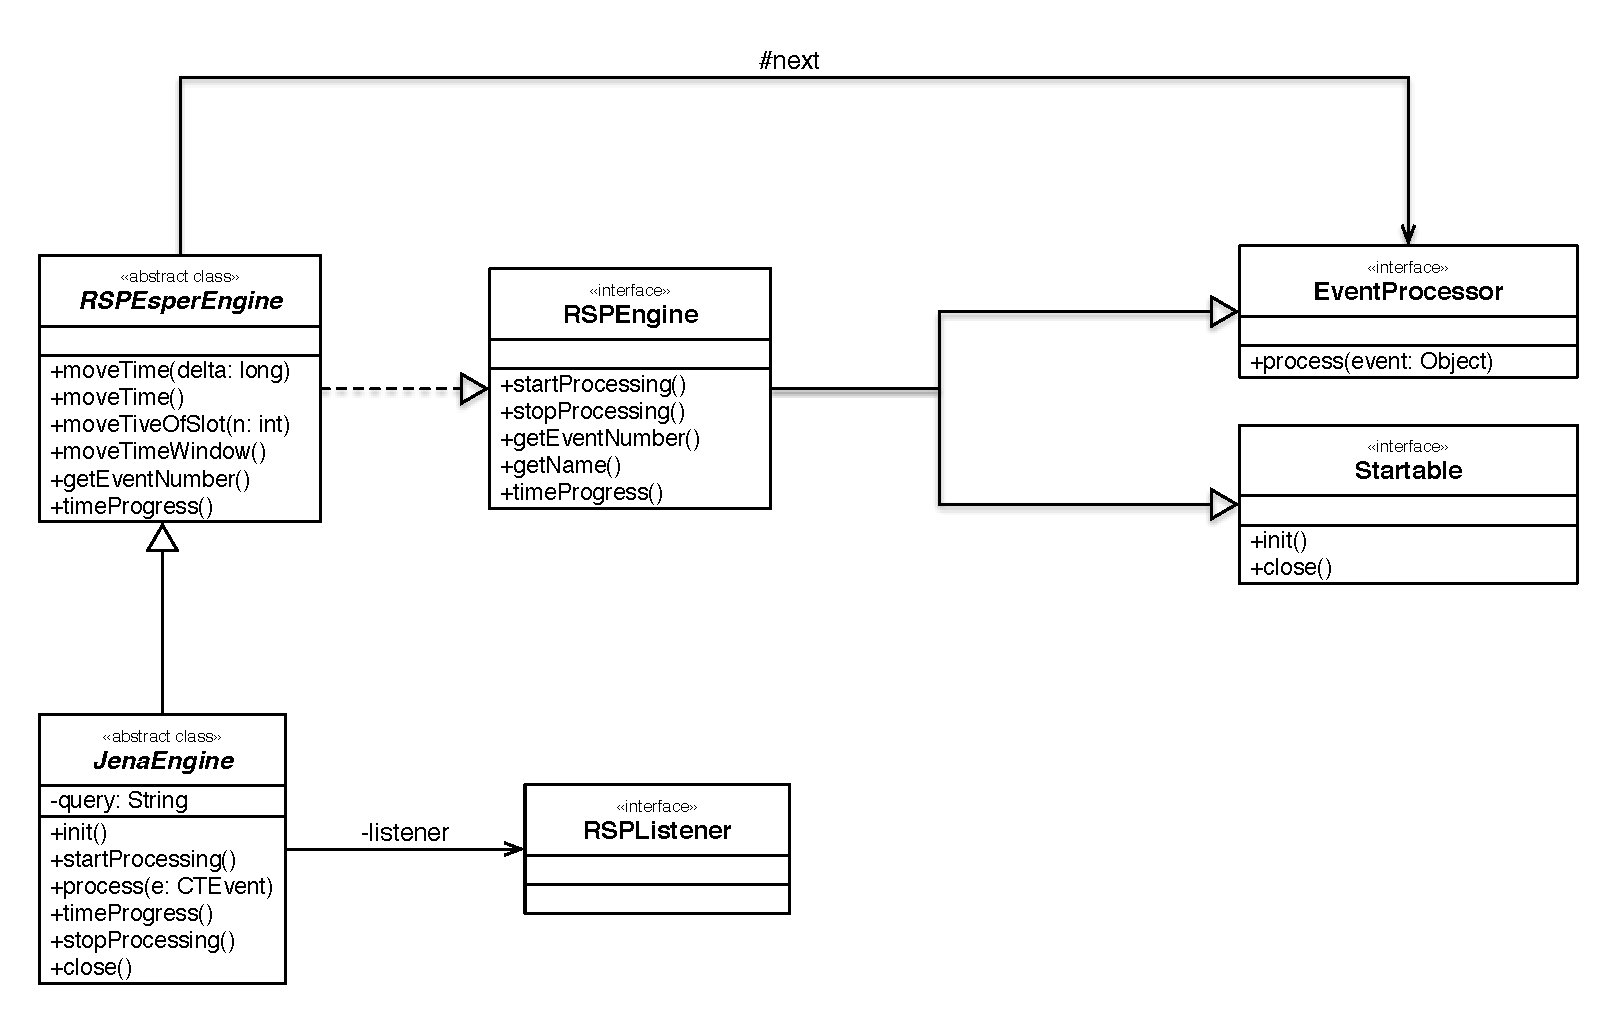
\includegraphics[width=\linewidth]{images/uml_baselines_general}
	\caption{RSPEsper Engine General UML Schema} 
  	\label{fig:uml_baselines_general}
\end{figure}

Figure \ref{fig:uml_baselines_general} shows the general implementation of the baselines: they  exploit the \textit{RSPEngine} interface, a proxy for an \textit{EventProcessor}, implementing the interface into the \textit{RSPEsperEngine} abstract class that includes the esper runtime. The next attributes, represents the general \textit{EventProcessor} which follows the RSPEngine in the \textsc{Test Stand} pipeline, it can be any modules which processes \textit{CTEvent}.

\begin{figure}[tbh]
  \centering
	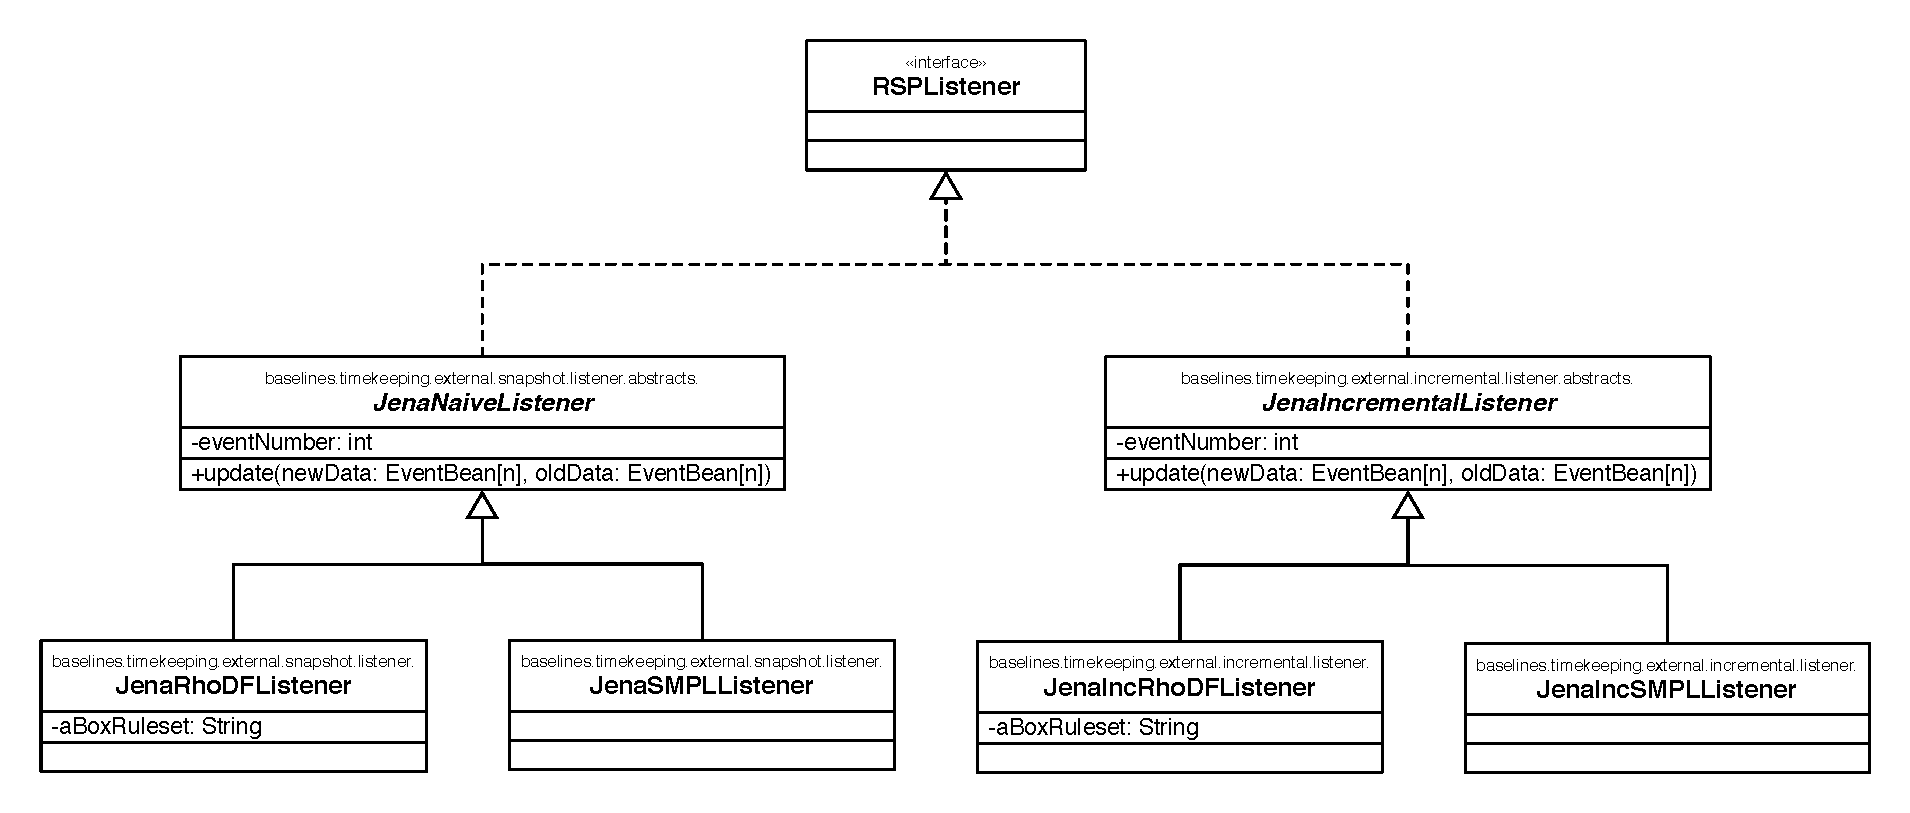
\includegraphics[width=\linewidth]{images/uml_baselines_listener}
	\caption{RSPListener UML Schema} 
  	\label{fig:uml_baselines_listener}
\end{figure}

In Figure \ref{fig:uml_baselines_general} is visible also the interaction between  the RSP Engine, represented by \textit{JenaEngine} abstract class, with the incoming \textit{CTEvent}. The engine is referencing the \textit{RSPListener} responsible to pipeline the Jena rule engine to the DSMS. 

\begin{figure}[tbh]
  \centering
	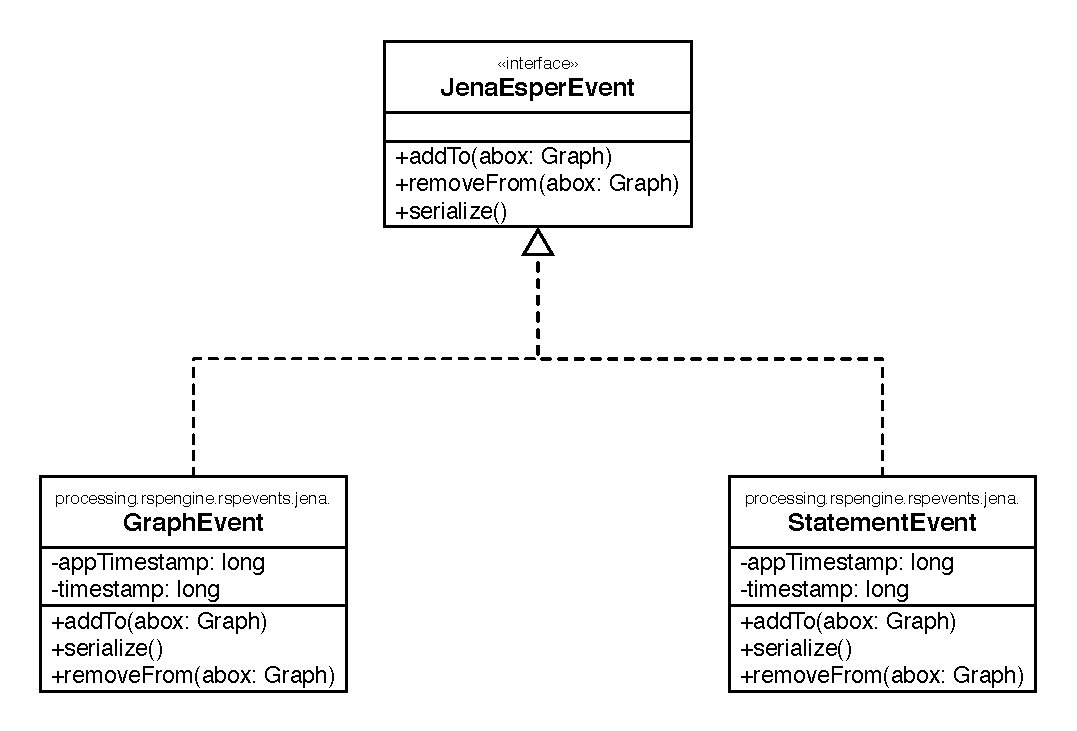
\includegraphics[width=0.5\linewidth]{images/uml_baselines_events}
	\caption{Esper-level events UML Schema} 
  	\label{fig:uml_baselines_events}
\end{figure}

Figure \ref{fig:uml_baselines_listener} shows the different implementations of the \textit{RSPListener}, which specify the reasoning approaches, Naive or Incremental as demanded by [R.15] (baseline relevance), according with the baseline design presented in Section \ref{sec:baselines}. Neither the \textit{JenaNaiveListener} or the \textit{JenaIncrementalListener} specify the entailment regime, which must be defined with specific implementations as it is visible in the Figure.



When a \textit{CTEvents} comes to the RSP Engine it will be transformed into the events handled by the DSMS, \ref{fig:uml_baselines_events}, this translation process influence the latency calculus. Once the processing is complete, the output of the RSP Engine is injected into an \textit{OUTCTEvent} and passed to the next \textit{EventProcessor} in the pipeline, which is the \textsc{Test Stand}. \textit{JenaEsperEvent} interface, as reported in Figure \ref{fig:uml_baselines_events} exposes methods to interact with the RDF model independently from the event implementation, which are Graph Based or Triple Based to cover baseline Relevance [R.15]. Moreover, Figure \ref{fig:uml_baselines_rel_listener_event} show how the \textit{JenaNaiveListener} and the  \textit{JenaIncrementalListener} handles the events which come form the DSMS trough the \textit{JenaEsperEvent} interface, for the case of Graph-based event representation (see Section \ref{sec:baselines} for event details). 

\begin{figure}[tbh]
  \centering
	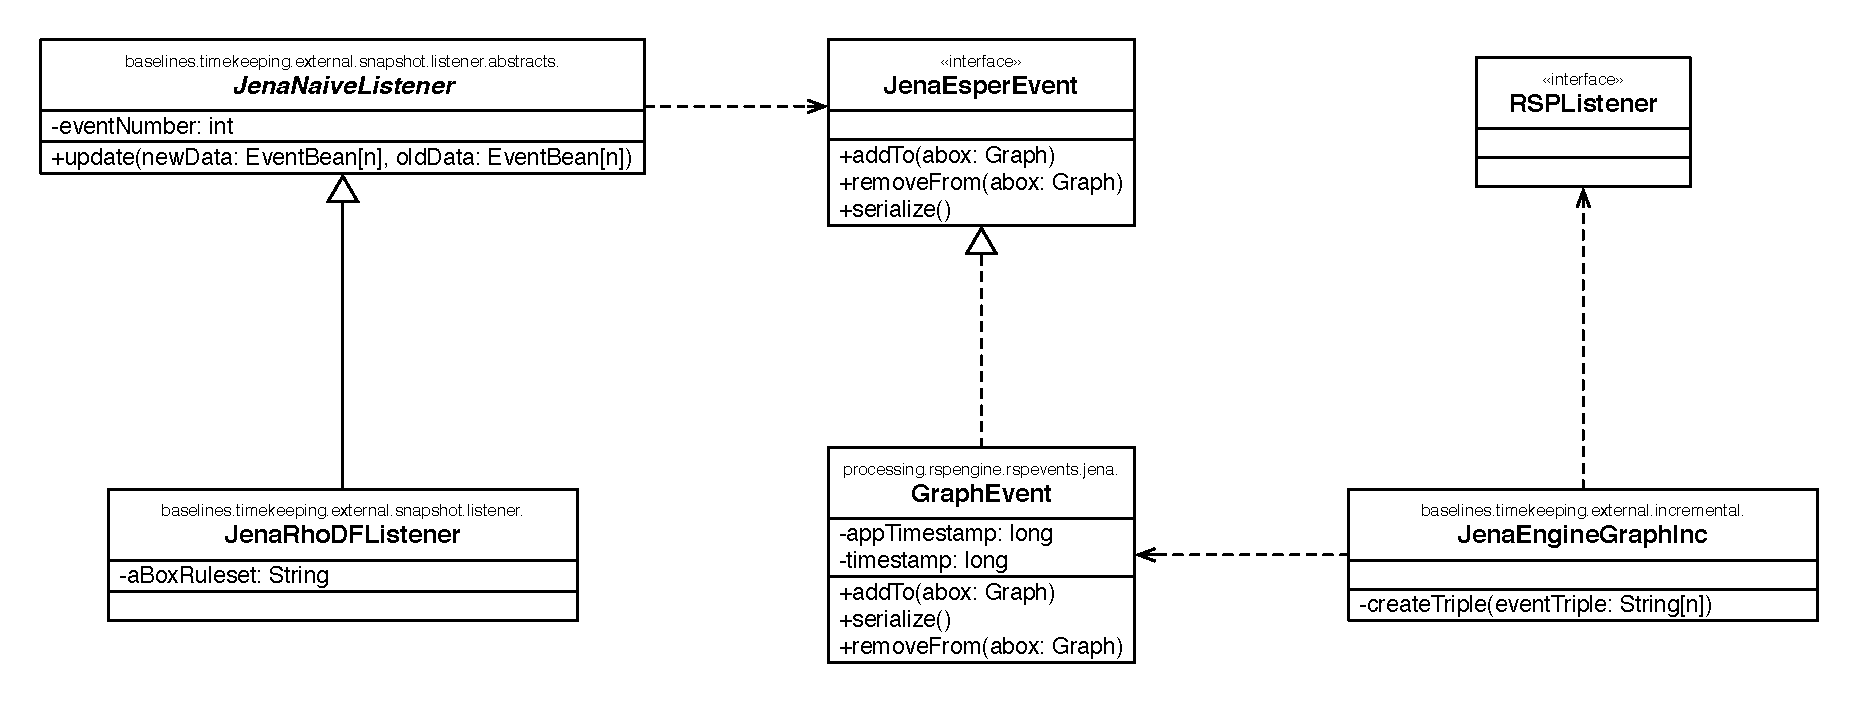
\includegraphics[width=\linewidth]{images/uml_baselines_rel_listener_event}
	\caption{RSPListener and events UML Schema} 
  	\label{fig:uml_baselines_rel_listener_event}
\end{figure}

This design allow the baselines to have a common design, sharing the majority of the code by splitting the different architectural elements. In this way we fulfil [R.16] which demands baseline Simplicity.


\section{Analyser}\label{sec:analyser-impl}

%R.9 allow qualitative analysis trough tools for result visualization



